\documentclass{article}
\usepackage{graphicx}
\usepackage{amsmath}
\usepackage{amsthm}
\usepackage{amssymb}
\usepackage{caption}
\usepackage{geometry}
\usepackage[style=numeric,bibstyle=numeric,backend=biber,natbib=true,maxbibnames=99,giveninits=true,uniquename=init]{biblatex}

\addbibresource{../bibliography.bib}
\title{Master's thesis topic description: Fine-tuned optical character recognition for dental fossil markings}
\author{Riikka Korolainen}
\date{014926659}

\begin{document}


\maketitle

\section{General problem area}

The research area of paleoecology studies past environments based on fossil remains.
Relying on ecological principles and statistical methods it is possible to learn various
traits of past ecosystems, such as what past climates were like, how species reacted 
to environmental changes and how early humans lived \cite{Faith_Lyman_2019}.

%paleoecology: data analysis on fossil data points

%what we are able to learn: makeup of species of past ecosystems, reactions
%of species to environmental changes, early human lifestyles \cite{Žliobaitė2023}

The National Museum of Kenya stores handwritten notes on found fossil specimens in the 
museum archives with the earliest being from the 1980's. The catalogue consists of 
approximately 90,000 unpublished specimens and an ongoing project is to digitize 
and publish the data. Accurately digitizing the data points will extend a paramount dataset 
to paleoecological research from the East African region and allow the data to be integrated 
to larger collections of fossil data, such as the NOW database \cite{Žliobaitė2023}.
%since 80's KNM has stored handwritten notes on found fossil specimens in 
%Kenya/Ethiopia. approx 4,500 pages with approx 50 specimens in the catalogue. 

%digitisation of hand-written fossil catalogues of the National Museum of Kenya
%digitizing these will make all fossil data analysis more accurate
%also allows integrating this data to larger collections of fossil data such as the NOW database \cite{Žliobaitė2023}

%digitisation with Azure AI Vision services done, but that model could 
%not read the special characters in the "element" column
Most of this digitisation effort was completed in a previous project using commercial 
Azure AI Vision services. However, this model could not read the special characters found 
in the data denoting tooth fragments. The aim of this thesis is to fine-tune an 
optical character recognition (OCR) model to recognize these markings. A sample of the markings and 
the Azure Vision output can be found in Figure \ref{image:data_sample}.

\begin{figure}[h]
    \centering
    \includegraphics*[scale=0.43]{sample.png}
    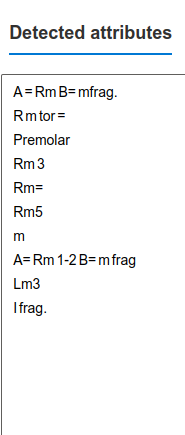
\includegraphics[scale=0.43]{azure_result.png}
    \caption{Sample from the tooth notation and corresponding Azure AI output}
    \label{image:data_sample}
\end{figure}

\section{Research questions}

The main research question is the following:

Which base model and fine-tuning method is most accurate for recognizing the special 
characters found in dental fossil notation?

The special characters consist of lower- and upper script numbers and letters with 
a line on top or underscoring. Additionally, there are multiple conventions for denoting the 
same tooth. For the fine-tuning, the methods are likely limited to few-shot transfer learning 
methods, since the data needs to be hand-labeled.

\section{Methodologies}

%Hand-label data or request from Kenya 

%Experiment: combinations of best OCR models + transfer techniques + 
%related problem solutions
%keep track of experiments with MLflow

%Train + store best method as a publicly available ML model. Submit to be 
%used by KNM + stakeholders. Also run model on catalogues, get out cleaned
%tooth records column

The thesis will consist of a literature review and an experimental section.
The literature review will consist of a synthesis of the relevant background 
information on deep learning, optical character recognition, transfer learning and 
paleoecology.
The main part of the literature review will consist of comparing
solutions to related problems of digitizing handwritten text that contains 
more unconventional characters. This part of the review can be divided into three partially overlapping review 
questions:

\begin{itemize}
    \item What is the best OCR model architecture?
    \item What is the best few-shot transfer learning method?
    \item Which solutions have previous works on related problems applied?
\end{itemize}

The goal of the literature review will be to choose a small set of solutions, which will be 
benchmarked in the experimental section. This part of the work will consist of attempting 
different combinations of approaches, and then comparing performance metrics. This will require a 
diligent experiment tracking system and hand-annotating data. The experiments will be performed 
using standard python data science libraries (pytorch, MLflow) and
 data from the fossil catalogues and specimen cards from the National Museum of Kenya. As a final deliverable,
 the fine-tuned model will be stored and made publicly available to be used by the museum.

\section{Key references}

\begin{itemize}
    \item \cite{li2021trocr} A promising base model for fine-tuning
    \item \cite{10478003} \cite{10.1145/3075645} \cite{10.1145/3542954.3542957} Solutions to similar problems
    \item \cite{9151144} A survey on optical character recognition methods 
    \item \cite{10.1145/3582688} A survey on few-shot transfer learning
    \item \cite{Faith_Lyman_2019} A thorough reference and bibliography on paleoecology
\end{itemize}

\section{Timeline and supervisors}

The aim is to finalize the work by the end of December, either to the steering group submission deadline on 19 December 2024 
or 23 January 2025. Supervisor: Indrė Žliobaitė, second reviewer: Kari Lintulaakso

\printbibliography
\end{document}